% Docker Meetup at MfN, 24 April 2018
% Running wikis at the Museum with Docker - past, present and future
% Alvaro Ortiz-Troncoso
% 
% Template:
% see https://en.wikibooks.org/wiki/LaTeX/Presentations

\documentclass{beamer}
\usepackage[utf8]{inputenc}
\usepackage{graphicx}
\usepackage{xcolor}

\definecolor{mfn_green}{HTML}{A1BF23}
\setbeamercolor{title}{fg=black}
\setbeamerfont{title}{family=\sffamily,series=\bf,size=\Large}
\setbeamercolor{frametitle}{fg=black}
\setbeamerfont{subtitle}{family=\sffamily,shape=\itshape}
\beamertemplatenavigationsymbolsempty
\setbeamertemplate{itemize item}{\color{mfn_green}$\blacktriangleright$}

%Running wikis at the Museum with Docker: past, present and future The Museum outputs exhibitions, science papers, conferences, and so much more. None of this would be %possible without cooperation between researchers, designers, organizers and of course admins and developers. Wikis were introduced at the Museum in 2014 as an %experiment to improve  cooperation within project teams. I'll talk about how Docker solves many of the problems of running a bunch of wikis on a string, and also %about pending questions we are currently trying to answer.
%I am a computer scientist and joined the Museum in 2014. I have worked at the Technische Universität Berlin and at Waag Technology & Society in Amsterdam.


\title
{Running wikis at the Museum with Docker}
\subtitle{past, present and future}
\author
{Alvaro Ortiz-Troncoso\inst{1}}
\institute % (optional)
{
  \inst{1}%
  Museum für Naturkunde Berlin
}
\date
{Docker Meetup at Museum für Naturkunde Berlin, 2018}
\subject{Computer Science}

\begin{document}
{
  \usebackgroundtemplate {
    \vbox to 30mm{\vfil\hbox to \paperwidth{\hfil
\includegraphics[width=30mm]{mfn_logo_klein.png}}\vfil}
  }
  \frame{\titlepage}
}

% The Museum
\begin{frame}
  \frametitle{Das Museum / \textcolor{mfn_green}{The Museum}}
  \begin{figure}
  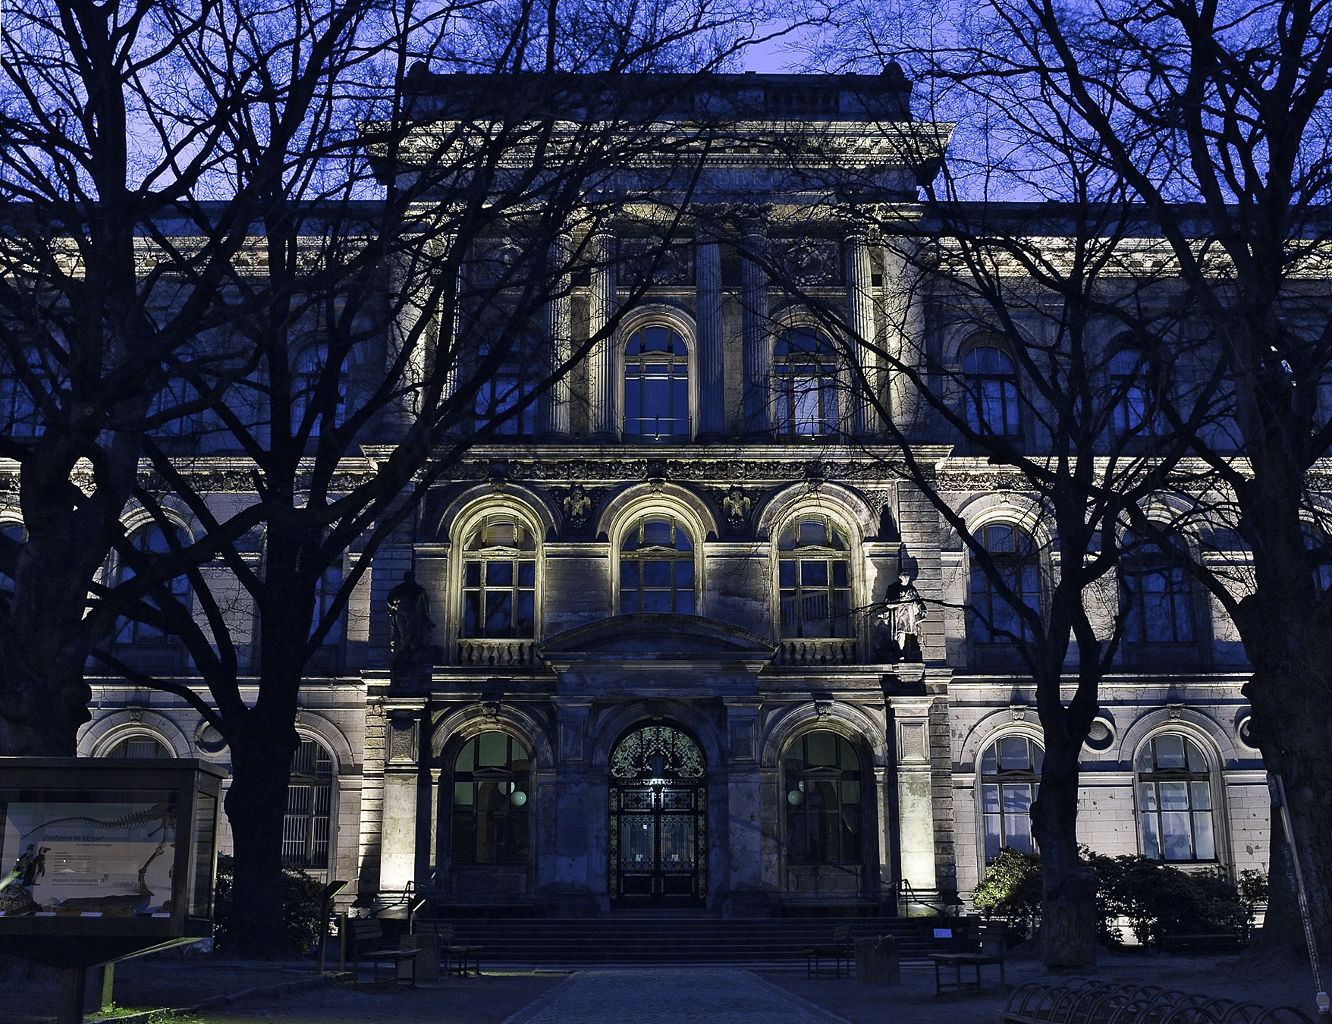
\includegraphics[height=70mm]{Gebaeude_Nacht.jpg}
  \end{figure}
  \begin{center}{\tiny \textcopyright Antje Dittmann, Museum für Naturkunde Berlin, 2009. CC-by-sa}\end{center}
\end{frame}

\begin{frame}
  \frametitle{Die Ausstellung / \textcolor{mfn_green}{The exhibition}}
  \begin{figure}
  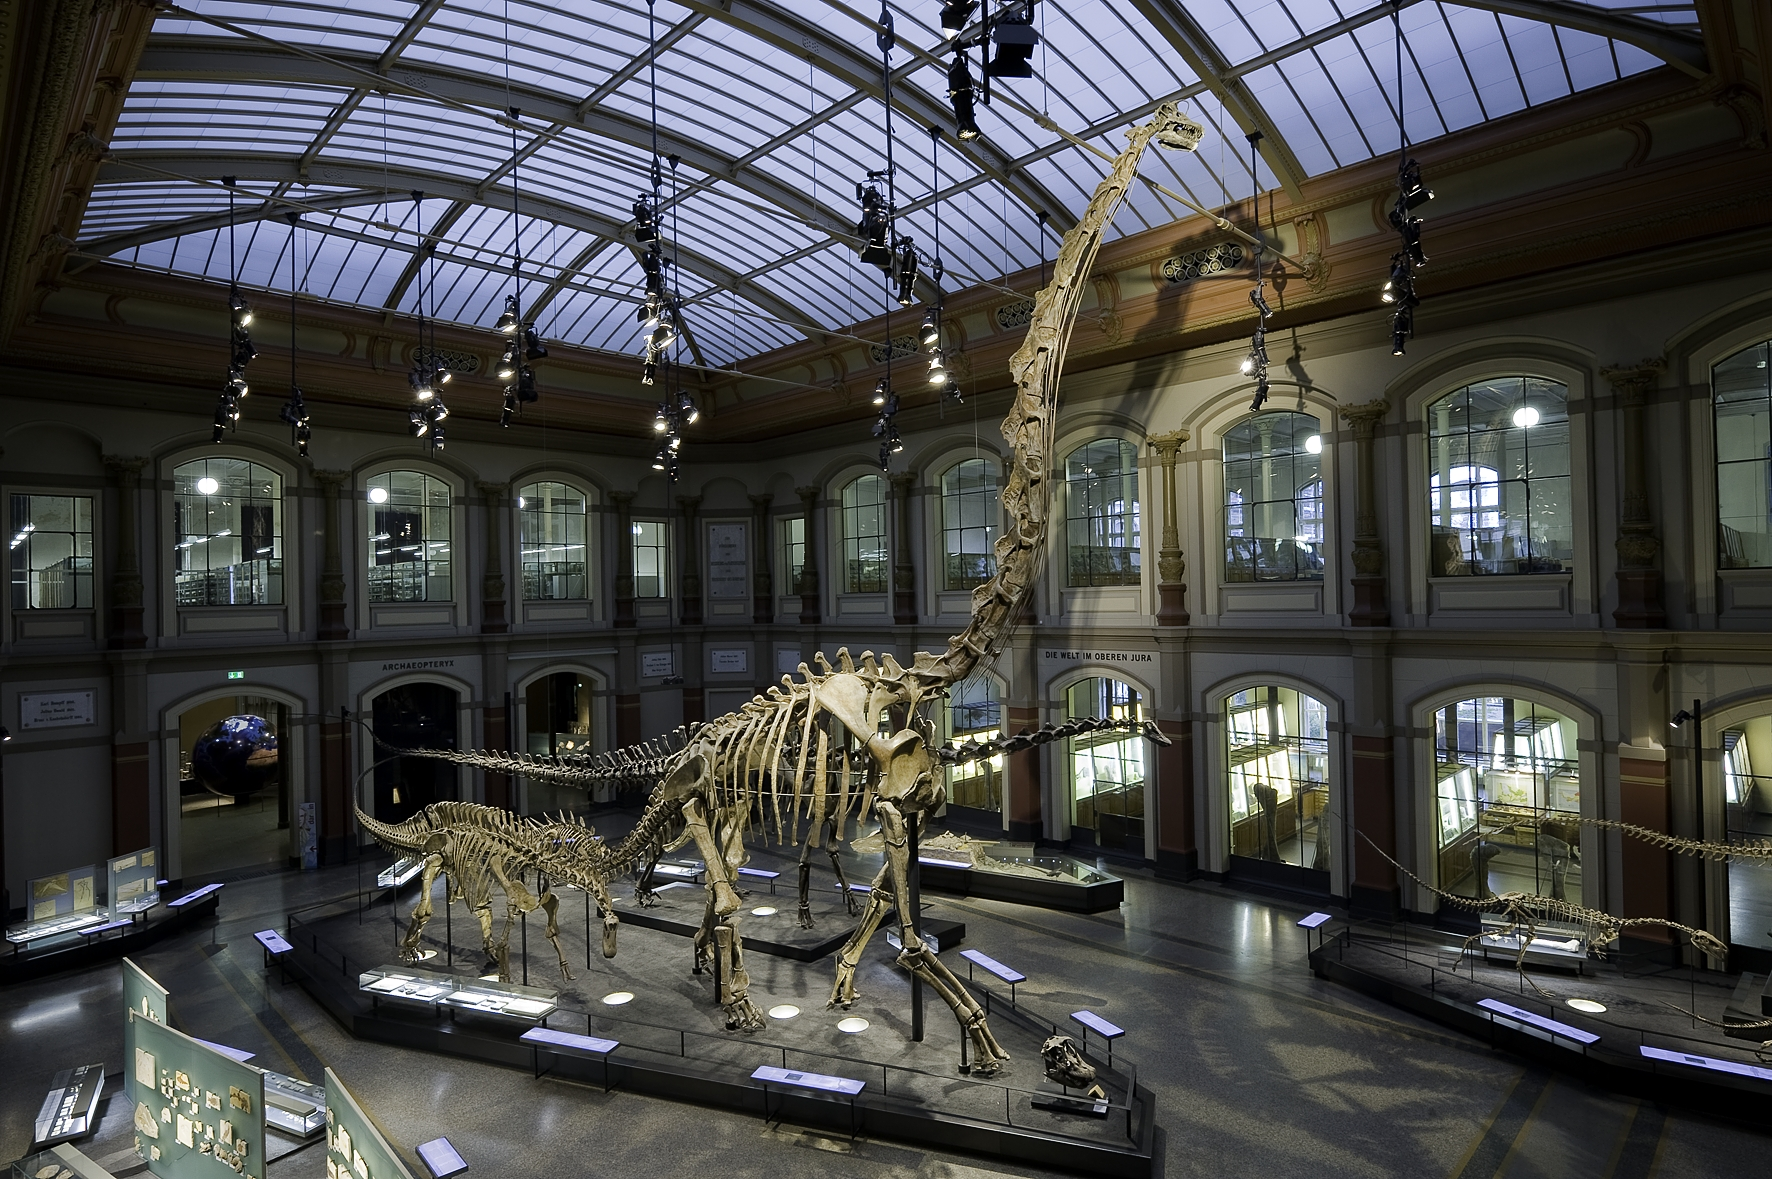
\includegraphics[height=70mm]{Brachiosaurus_02_15cm.jpg}
  \begin{center}{\tiny \textcopyright Antje Dittmann, Museum für Naturkunde Berlin, 2009. CC-by-sa}\end{center}
  \end{figure}
\end{frame}

\begin{frame}
  \frametitle{Forschungsprojekte / \textcolor{mfn_green}{Research projects}}
  \begin{figure}
  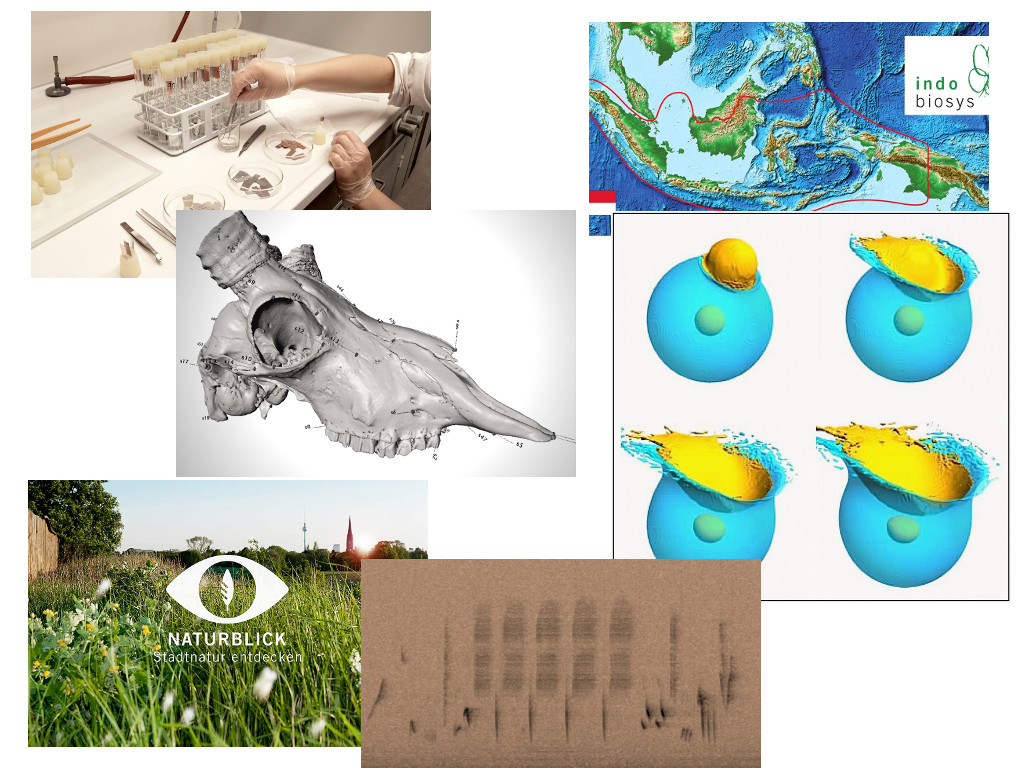
\includegraphics[height=70mm]{Forschung.jpg}
  \end{figure}
\end{frame}

{
\setbeamercolor{background canvas}{bg=mfn_green}
\setbeamercolor{frametitle}{fg=black}
\begin{frame}
  \frametitle{Was macht ein Projekt aus? /\\ \textcolor{white}{What does it take to launch a project?}}
  \begin{figure}
  \includegraphics[height=70mm,trim=4 4 4 4,clip]{Projekt.png}
  \end{figure}
\end{frame}
}

\begin{frame}
  \frametitle{Kooperation / \textcolor{mfn_green}{Cooperation}}

  \begin{itemize}
  \item{Gemeinsames Verständnis der Projektziele}
  \item{Innerhalb des Zeitrahmens zum Ergebnis kommen}
  \item{Den Kostenrahmen nicht überschreiten - Effizient arbeiten}
  \end{itemize}
  
  \begin{itemize}
  \item{\textcolor{mfn_green}{Common understanding of project goals}}
  \item{\textcolor{mfn_green}{Deliver on time}}
  \item{\textcolor{mfn_green}{Be efficient to finish within budget}}
  \end{itemize}
\end{frame}

% The past
\begin{frame}
  \frametitle{In der Vergangenheit / \textcolor{mfn_green}{In the past}}
  \begin{figure}
    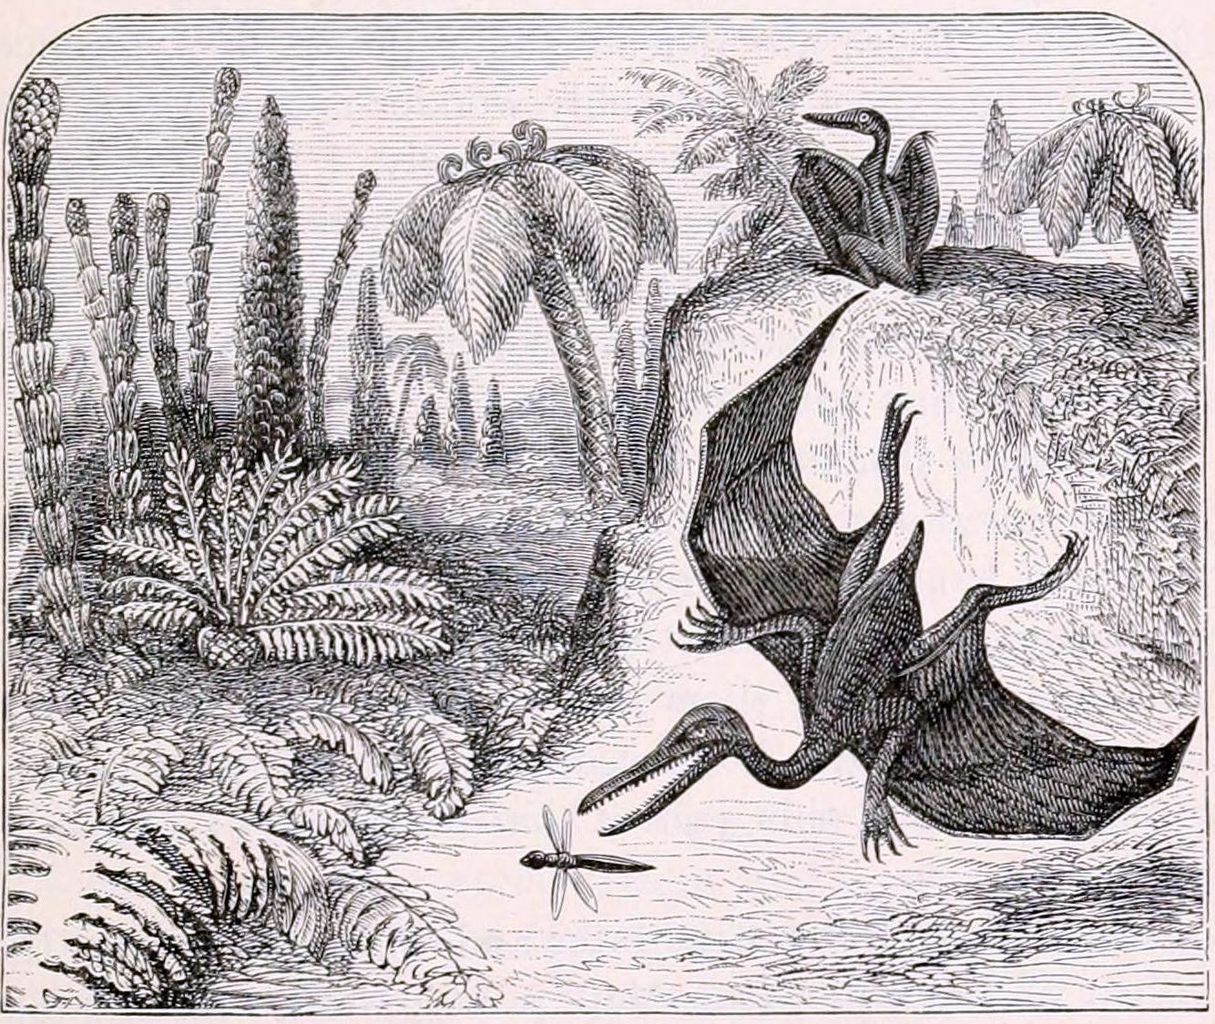
\includegraphics[height=70mm]{Ideal_Landscape_of_a_Prehistoric_Age.jpg}
  \end{figure}
  \begin{center}{\tiny Quackenbos, J.D., 1886. \textit{Illustrated School History of the World}. D. Appleton.}\end{center}
\end{frame}

{
\setbeamercolor{background canvas}{bg=mfn_green}
\setbeamercolor{frametitle}{fg=black}
\begin{frame}
  \frametitle{Word\textsuperscript{\tiny\textregistered} .doc Hölle /
    \textcolor{white}{Word\textsuperscript{\tiny\textregistered} .doc hell}}
  \begin{figure}
  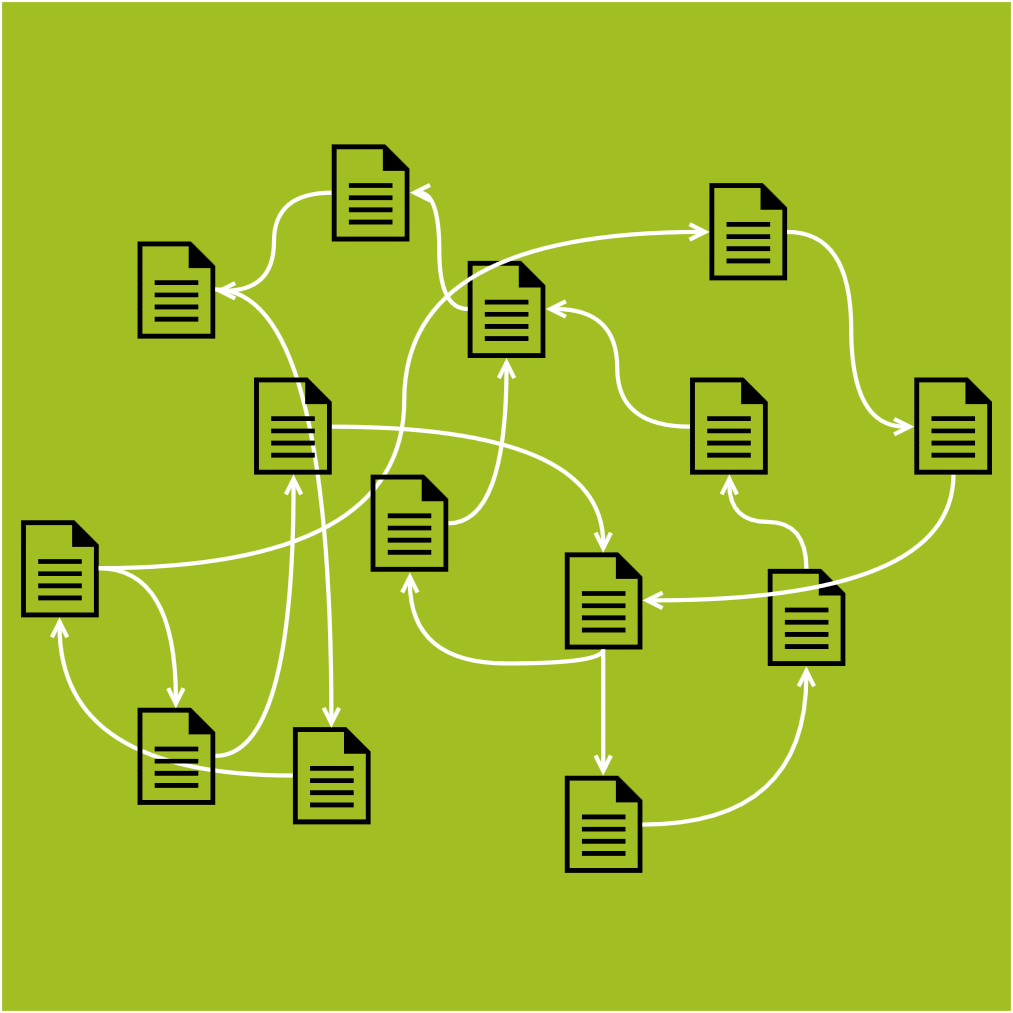
\includegraphics[height=70mm,trim=4 4 4 4,clip]{Docs.png}
  \end{figure}
\end{frame}
}

\begin{frame}
  \frametitle{Nichts gegen Word\textsuperscript{\tiny\textregistered} aber... / \\
    \textcolor{mfn_green}{Absolutely nothing against Word\textsuperscript{\tiny\textregistered}, however, ...}}
  \begin{itemize}
  \item{Keine Versionierung: wer hat die Endfassung?}
  \item{Kein Dokumentverlauf: wer hat was geschrieben?}
  \item{Proprietäre Software: Anbieterabhängigkeit}
  \end{itemize}
  
  \begin{itemize}
  \item{\textcolor{mfn_green}{No versioning: who has the final version}}
  \item{\textcolor{mfn_green}{No document history: who wrote what?}}
  \item{\textcolor{mfn_green}{Proprietary software: vendor lock-in}}
  \end{itemize}
\end{frame}


% The present
\begin{frame}
  \frametitle{This is the first slide}
  % Content goes here
\end{frame}

% The future
\begin{frame}
  \frametitle{This is the first slide}
  % Content goes here
\end{frame}


\end{document}


